The PC environment had morphed significantly between the development of Wolfenstein 3D in 1991 and the development of Doom in 1993. The previous "recommend configuration" based on an Intel 386 CPU with 2~MiB of RAM and a VGA graphic card was no more.\\
\par
The "new" typical PC still had six subsystems \circled{1}~Inputs, \circled{2}~CPU, \circled{3}~RAM, \circled{4}~Bus, \circled{5}~Video~output, and \circled{6}~Audio~output together forming a pipeline.\\
\par
\pngdrawing{pc_components}{The six components of an IBM PC.}
\par
Only each of these sub-systems had become faster or increased its capacity. Before describing each components in details, it is important to remind the reader that despite these improvements, the IBM PC was still not something built for video games. These were machine originally designed to do word processing, spreadsheet and sometimes display a static graph. The goal was never to have something on screen refreshing at 70Hz\footnote{The VGA refresh rate was 70Hz contrary to today ubiquitous 60Hz.}. Not to mention the pricetag where a top of line machine fetched close to \$13,000 adjusted to inflation.\\
\par Looking back it seem hard to believe studios focused on producing titles for these expensive and seemingly less capable machines when it came to video games. With a CPU unable to floating-point, a graphic system with no double buffering capabilities, and a sound system only capable of irritating "beeps" a PC was unappealing at best and probably less propice to profit, especially compared to cheaper systems such as the Super Nintendo, the Sega Genesis, or the Neo-Geosystems\footnote{At introduction, the SNES and the SEGA Genernis were both priced at US\$199 while the top of the line Neo-Geo was US\$649.99.} which were designed from the ground up for video games. \\
\par
Obviously, given the title of the book you have in your hands, with a few software tricks the hardware of the PC was capable of more than what it was designed for. But I felt the hardware chapter should do it best not outline the limitations as well as the bottleneck of the available metal.\\
\par


\cfullimage{ibm_ps1_top}{IBM PS1 featuring an Intel 486. Notice how the ad emphasis static screen office apps. Also notice the standard 14" CRT which probably weighted close to 20 pounds!}

\cleartoleftpage
 The best way to get an overview is to look at the best selling motherboard of the year 1993, the PX486P3 by QDI Computer, Inc\footnote{Again, a canadian company :) !}.\\
\par

\cfullimage{PX486P3/b-486-px486p3_romain}{Motherboard PX486P3 by QDI Computer, Inc}
\par
The most prominent novelty is of course the heart of the computer, the Intel i486 CPU. Yet a closer looks reveals many more features which would be of paramount importance for the design of \doom.\\
\par 
If the black extension connectors show the traditional ISA bus ports, a 8 bit one (\circled{1}), two dual slot 16 bit (\circled{2}) we can also see a new type of connector with three slots (\circled{3}). These are VBL\footnote{Video Local Bus.}, a new type of bus up to 20x faster than ISA.\\
\par
 Next in the upper right (\circled{5}), a new type of RAM had found its way into these new PC. In black, eight chips of Static RAM offered 256 KiB acting as "cache", a new system to prevent CPU starvation. see large rows of black chips, a new type of RAM called sRAM\footnote{Static RAM}, up to 10x faster than dRAM\footnote{Dynamic RAM} aiming at avoiding CPU stalls\footnote{SRAM was expensive and took a lot of space. Despite their size compared to the DRAM (in white), the eight chips could only stored 256 KiB with 20ns access time.}. \\
\par
\drawing{px486p3}{Components diagram of the PX486P3.}
\par
The main memory system had grown in capacity, speed and complexity. Thanks to a sharp decline in manufacturing price, the standard DRAM installed (\circled{4}) had doubled to 4MiB\footnote{\doom would not run on PC equipped with "only" 2 MiB}.\\
\par

\begin{center}
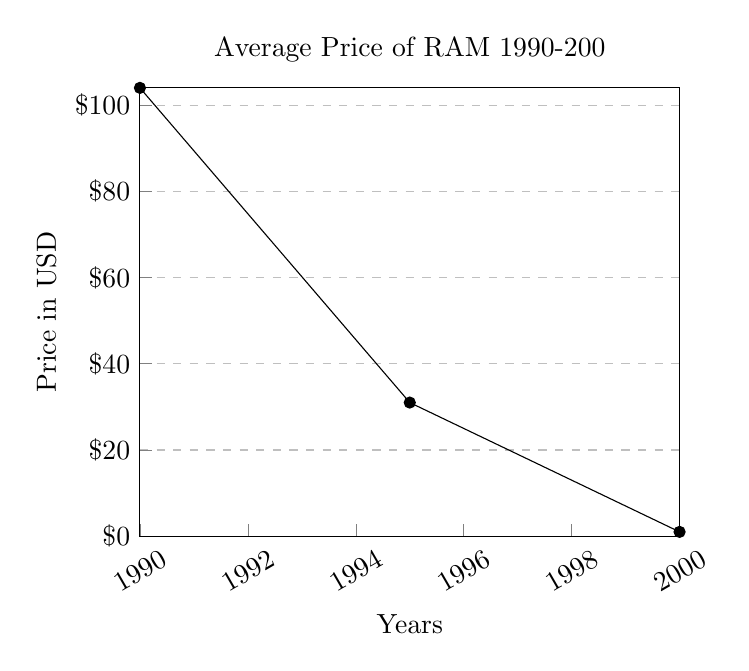
\begin{tikzpicture}

\begin{axis}[
    title={Average Price of RAM 1990-200},
    xlabel={Years},
    xtick pos=left,
    ytick pos=left,
    ylabel={Price in USD},
    yticklabel={${\$\pgfmathprintnumber{\tick}}$},
    xticklabel style={ rotate=30,},
    xticklabel style={/pgf/number format/1000 sep=},
    xmin=1990, xmax=2000,
    ymin=0, ymax=104,
    %xtick={0,20,40,60,80,100},
    %ytick={0,20,40,60,80,100,120},
    legend pos=north west,
    ymajorgrids=true,
    grid style=dashed,
]
 
\addplot[
    color=black,
    mark=*,
    ]
    coordinates {
    (1990,104)(1995,31)(2000,1)
    };
    %\legend{CuSO$_4\cdot$5H$_2$O}
 
\end{axis}
\end{tikzpicture}
\end{center}

% \begin{enumerate}
% \item RAM prices had dropped significantly. The standard 2 MiB was not a whooping 4 MiB. 
% \item Bandwidth hungry GUI and had lead motherboard manufacturers to come up with a faster bus called VLB.
% \item The sound generator ecosystems was even more fragmented than before with more and more manufacturer producing sound cards.
% \item Not visible on the drawing, the operating system shortcomings were being addressed by independent developers via something called "DOS eXtenders".
% \item Unsurprisingly the impossible to program VGA was still the standard but manufacturers were now competing to produce the faster DACs and \fixme{"RAMDAC"}?.
% \item CACHE
% \end{enumerate}


Back then, it was a fair assumption to assume the next PC would have twice the processing power and twice the RAM capacity.
\par
\break





